\documentclass[11pt]{article}
\renewcommand{\baselinestretch}{1.05}
\usepackage{amsmath,amsthm,verbatim,amssymb,amsfonts,amscd, graphicx}
\usepackage{blindtext}

\usepackage{caption}
\usepackage{enumitem}

%Additional Packages
\usepackage{enumitem}
\usepackage{graphics}
\usepackage{float}
\graphicspath{ {images/} }
%\usepackage[framed]{mcode}
\usepackage{hyperref}
\hypersetup{
	colorlinks=true,
	linkcolor=blue,
	filecolor=magenta,      
	urlcolor=cyan,
}

\topmargin0.0cm
\headheight0.0cm
\headsep0.0cm
\oddsidemargin0.0cm
\textheight23.0cm
\textwidth16.5cm
\footskip1.0cm
\theoremstyle{plain}
\newtheorem{theorem}{Theorem}
\newtheorem{corollary}{Corollary}
\newtheorem{lemma}{Lemma}
\newtheorem{proposition}{Proposition}
\newtheorem*{surfacecor}{Corollary 1}
\newtheorem{conjecture}{Conjecture} 
\newtheorem{question}{Question} 
\theoremstyle{definition}
\newtheorem{definition}{Definition}

\usepackage{indentfirst}
%\renewcommand{\thesubsubsection}{\thesubsection.\alph{subsection}}

\newcommand{\floor}[1]{\lfloor #1 \rfloor}

%SETUP PSUEDOCODE
\usepackage{tcolorbox}


%SETUP AtxMEGA128A1U
\usepackage{listings}

\usepackage{xcolor}
\definecolor{bluekeywords}{rgb}{0.13,0.13,1}
\definecolor{greencomments}{rgb}{0,0.5,0}
\definecolor{turqusnumbers}{rgb}{0.17,0.57,0.69}
\definecolor{redstrings}{rgb}{0.5,0,0}

\lstdefinelanguage{atxmega128a1u}{
	morekeywords={include, ,org, rjmp, CSEG, db, equ, DSEG, ldi, lds, sts,  breq, brne, and, cp, cpi, push, pop, ret},
	keywordstyle=\color{bluekeywords},
	sensitive=false,
	morecomment=[l][\color{greencomments}]{;},
	morecomment=[s][\color{greencomments}]{{/*}{*/}},
	morestring=[b]",
	stringstyle=\color{redstrings}
}

\lstnewenvironment{asmlisting}{
	\lstset{
		frame=single,
		language=atxmega128a1u,
		basicstyle=\ttfamily,
		breaklines=true,
		columns=fullflexible
	}
}
{}
%
% START OF DOCUMENT
%
\begin{document}
\captionsetup[figure]{labelfont=bf} 

\title{Lab 2}
\author{\textbf{Michael Arboleda}\\Lab Section: 7F34}
\maketitle
%
% PRELAB QUESTIONS
%
\section*{b. Answers to all pre-lab questions}
\begin{enumerate}[label={\arabic*)},font={\color{red}\bfseries}]
	%
	%1
	%
	\item How many TC0 channels are necessary to control all three LEDs in the uPAD’s RGB LED
	\\[0.8ex]
	\textbf{ANS: } 3. One for red, one for green, one for blue
	%
	%2
	%
	\item What would happen if the RGB period was FFFF instead
	of FF?
	\\[0.8ex]
	\textbf{ANS: } The amount of cycles need restart is higher. Thus the time for a LED to be ion is bigger
\end{enumerate}
%
% PROBLEMS ENCOUNTERED
%
\section*{c. Problems Encountered} 
My overflow interrupt would not work, even tho the Flag did go off. I changed the location of the .ORG and it worked 
%
% FUTURE WORK
%
\section*{d. Future Work/Applications}
IT is clear why interrupts and timer/counters are important. In the future I can learn about the different types of interrupts, not just external and overflow. 
%
% SCHEMATICS
%
\section*{e. Schematics}
N/A
%
% PSEUDOCODE
%
\newpage
\section*{g. Pseudocode/Flowcharts}
%
% PSEUDOCODE PART A
%
\textbf{\textcolor{blue}{Pseudocode for lab3a.asm:}}
\begin{tcolorbox}
\begin{verbatim}
MAIN:

    * Equate numbers
    * Set registers to hold constants

    * Call Change_CLK_32HZ subroutine
    * Remap Pin Ports
    * Set PORT D/LED to output
    * Invert Port D
    * Set TOP of PWM
    * Set up Control D for port D
    * Set up Control B for port D
    * Set up Compare Chanel
    * Set up Control D for port D

WHILE(TRUE){}
END


SUBROUTINE Change_CLK_32HZ
    * Enable the new oscillator

    WHILE(OSC FLAG not set){}

    * Write the “IOREG” signature to the CPU_CCP reg
    * Select the new clock source in the CLK_CTRL reg
    * Return to program
\end{verbatim}
\end{tcolorbox}
%
% PSEUDOCODE PART B
%
\newpage
\textbf{\textcolor{blue}{Pseudocode for lab3b.asm:}}
\begin{tcolorbox}
\begin{verbatim}
MAIN:

* Equate numbers
* Set registers to hold constants
* Call Change_CLK_32HZ subroutine

* Set up LEDS and Switches

* Set up External interrupt

SUBROUTINE BLUE_PWM:
* Remap Pin Ports
* Set PORT D/LED to output
* Invert Port D
* Set TOP of PWM
* Set up Control D for port D
* Set up Control B for port D
* Set up Compare Chanel
* Set up Control D for port D


ISR inc_display:
* INCREMENT counter
* Display on LED
\end{verbatim}
\end{tcolorbox}	
%
% PSEUDOCODE PART C
%
\newpage
\textbf{\textcolor{blue}{Pseudocode for lab3c.asm:}}
\begin{tcolorbox}
\begin{verbatim}
MAIN:

* Equate numbers
* Set registers to hold constants
* Call Change_CLK_32HZ subroutine

* Set up LEDS and Switches

* Set up External interrupt

WHILE(TRUE){
* Toggle LED
}

END

ISR overflow_logic:
IF(BUTTON PRESSED){
* INCREMENT COUNT
* DISPLAY COUNT
}
* Disable Timer interrupt
* Disable Timer
* Enable external interrupt
* Clear Interupts flags

ISR ext_int_logic
* Disable external interrupt
* Initialize Timer and Timer interrupt
* Clear Flags

SUBROUTINE SET_COUNTER: 
* Set TOP(PER) for counter

SUBROUTINE SET_COUNTER_INT:
* Set interrupt for counter
* Run Counter     	


\end{verbatim}
\end{tcolorbox}





%
% PSEUDOCODE PART D
%
\newpage
\textbf{\textcolor{blue}{Pseudocode for lab3d.asm:}}
\begin{tcolorbox}
\begin{verbatim}
MAIN:

* Equate numbers
* Set registers to hold constants
* Call Change_CLK_32HZ subroutine

* Set up LEDS and Switches

* call PWM_setup

* Set up PORT F interupt 

While(TRUE){
	* Toggle LED
	
	** Wait for external interupt **
	** Run ext_int_logic ISR
	*** Wait for overflow interupt
	*** Run overflow_logic ISR	
	*** Wait for 2nd overflow interupt
	*** Run overflow_05_logic ISR
}

END

SUBROUTINE PWM_setup:
* Remap Ports
* Set CTRLs

ISR ext_int_logic:
* Disable external interrupt
* call STOP_05_COUNTER Subroutine
* Initialize Timer and Timer interrupt
* Clear Interupts flags

SUBROUTINE STOP_05_COUNTER:	
* Disable Timer interrupt
* Disable Timer

SUBROUTINE SET_COUNTER:
* Set up TOP (PER)
\end{verbatim}
\end{tcolorbox}


\begin{tcolorbox}
\begin{verbatim}

SUBROUTINE SET_COUNTER_INT:
* Set Interupt config
* Start counter

ISR overflow_logic:
If(button is still held){
	* increment external button counter
	* Display erternal button on LEDs 
}

* Call subroutine STOP_COUNTER
* Reset switcher counter
* Enable external interupt
* Set up .05sec timer and interrupt
* Set up compare chanel
* Clear interrupt flags

SUBROUTINE STOP_COUNTER
* Disable Timer interrupt
* Disable Timer

SUBROUTINE SET_05_COUNTER:
* Set up TOP (PER)

SUBROUTINE SET_05_COUNTER_INT:
* Set Interupt config
* Start counter

ISR overflow_05_logic	
* Call SET_COMPARE_CH

SUBROUTINE SET_COMPARE_CH:
* Restart counter for PWM_setup
* Set Color Reg
IF(Switches counter = 0){
	* Use first color of pattern
	* Set Switches counter to 1
}
ELSE{
	* Use 2nd color of pattern
	* Set Switches counter to 0
}	
* Set up Compare Chanel A, B, C
* Run Counter
\end{verbatim}
\end{tcolorbox}

\begin{tcolorbox}
\begin{verbatim}

SUBROUTINE Set_Pattern:
IF(Counter mod 4 = 0){
	* Set all colors to off
}
ELSE IF(Counter mod 4 = 1){
	* Set UF colors
}
ELSE IF(Counter mod 4 = 2){
	* Set Holiday Colors
}
ELSE IF(Counter mod 4 = 3){
	* Set Hulk Colors
}
\end{verbatim}
\end{tcolorbox}







\newpage
\section*{h. Program Code}
\textbf{\textcolor{blue}{Code for lab3a.asm:}}
\lstinputlisting[language=atxmega128a1u, frame=single]{lab3a.asm}
\newpage
\textbf{\textcolor{blue}{Code for lab3b.asm:}}
\lstinputlisting[language=atxmega128a1u, frame=single]{lab3b.asm}
\newpage
\textbf{\textcolor{blue}{Code for lab3c.asm:}}
\lstinputlisting[language=atxmega128a1u, frame=single]{lab3c.asm}
\newpage
\textbf{\textcolor{blue}{Code for lab3d.asm:}}
\lstinputlisting[language=atxmega128a1u, frame=single]{lab3d.asm}


\section*{i. Appendix}
\begin{figure}[H]
	\centering
	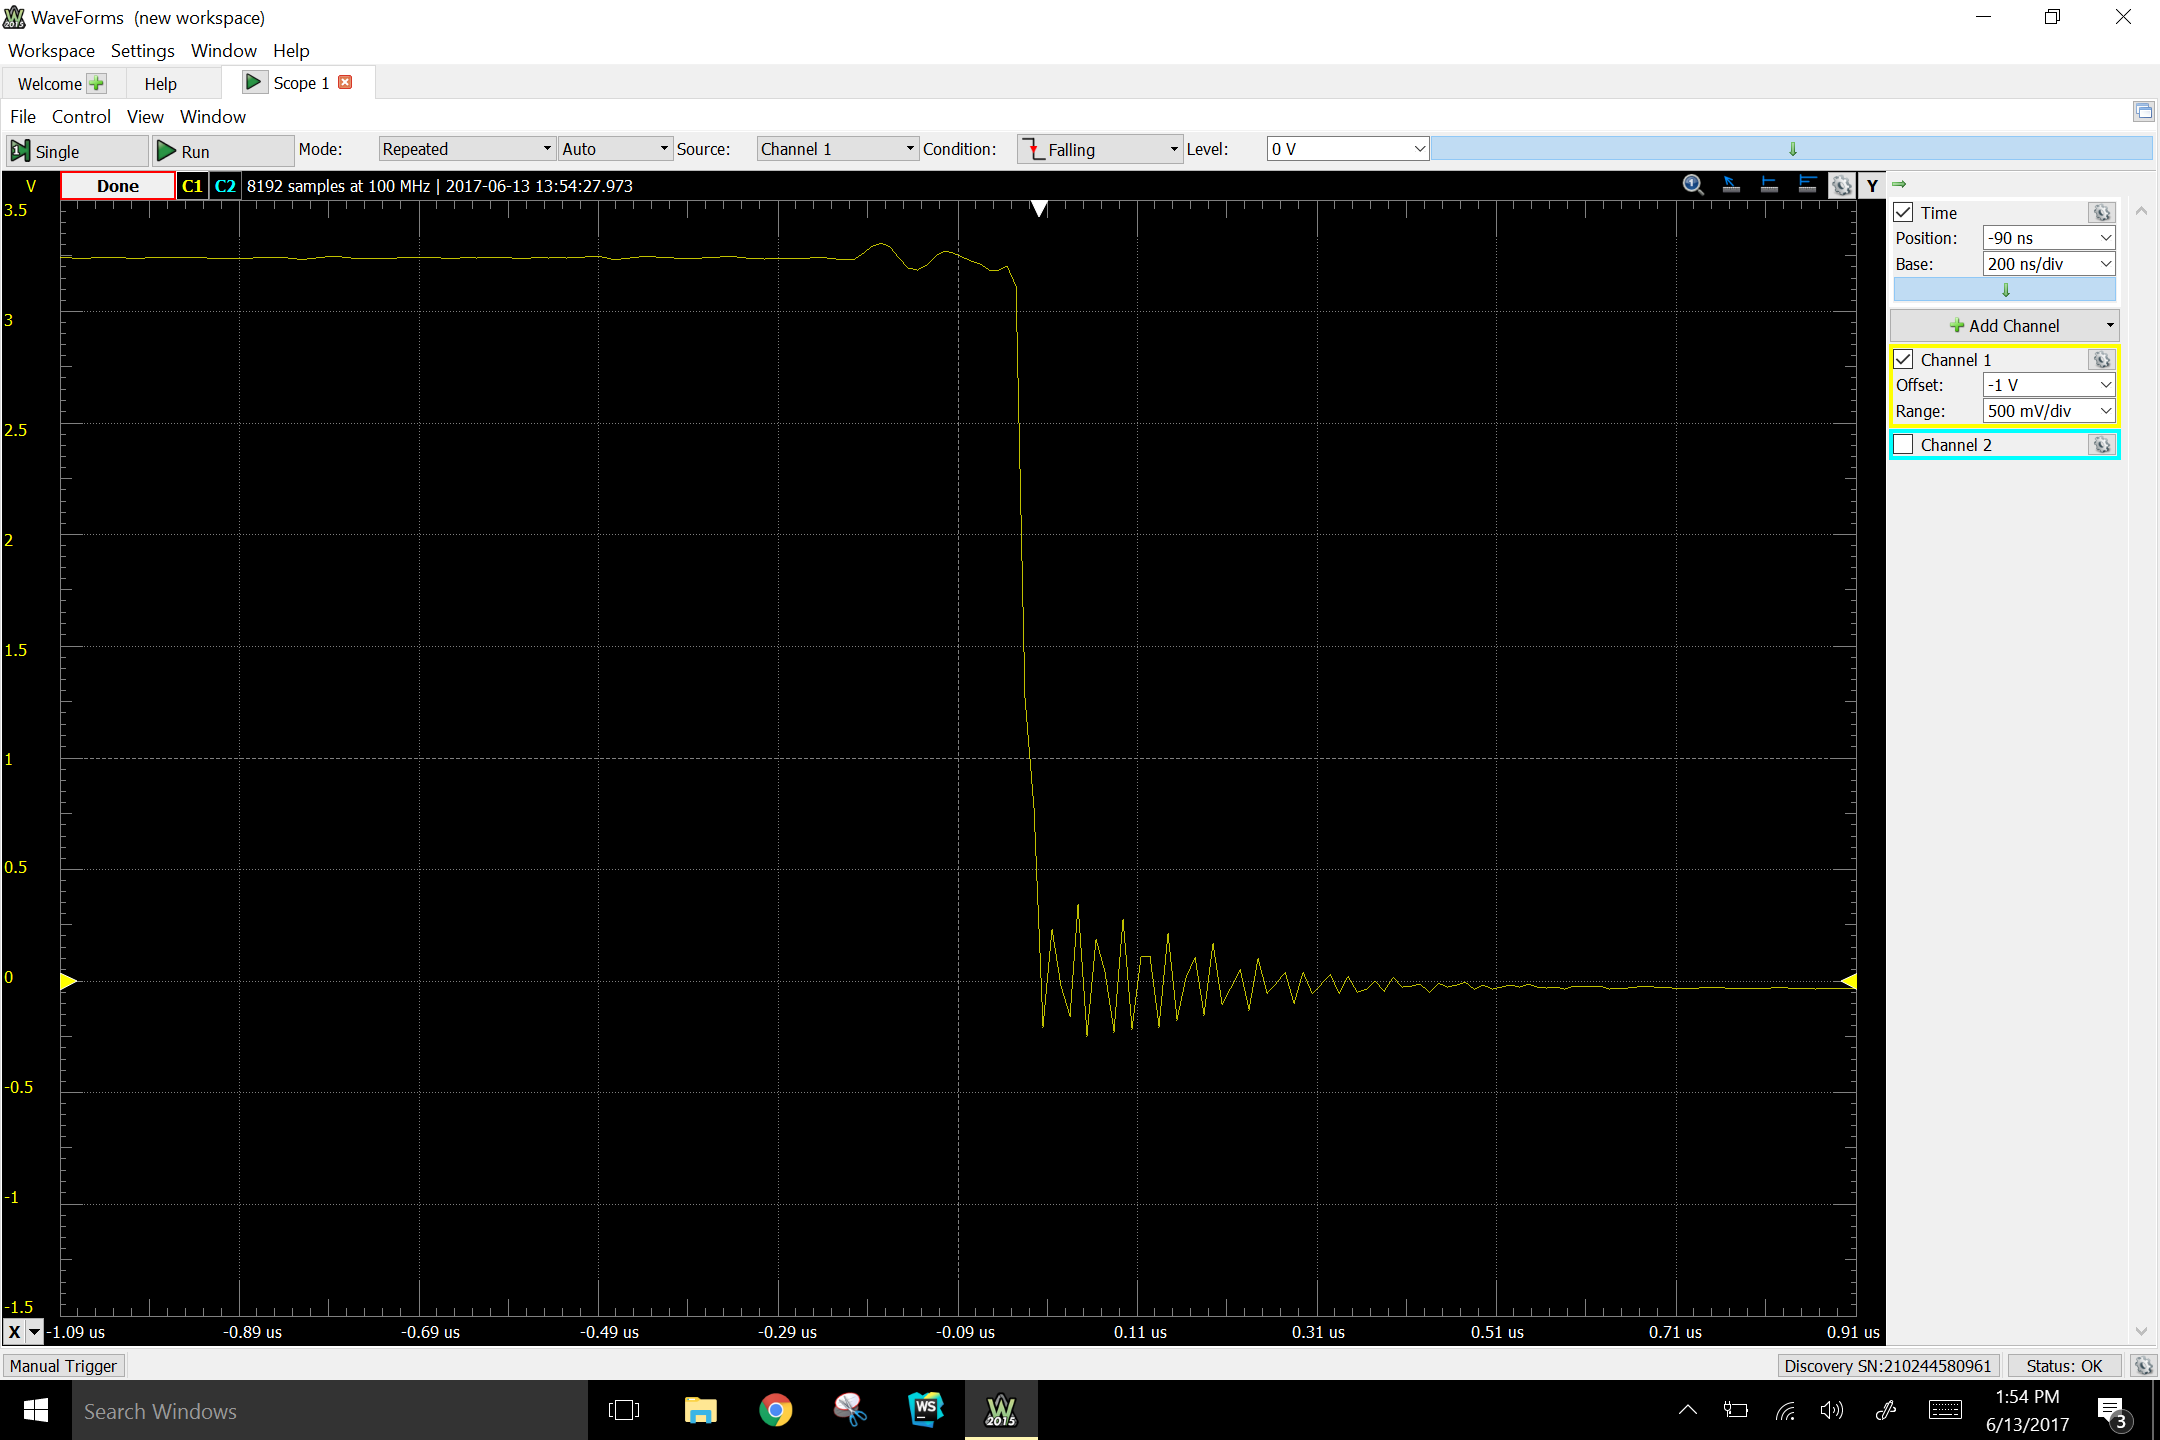
\includegraphics[width=\textwidth]{3a}
	\label{fig:c}
	\caption{DEBOUNCE FALLING EDGE 1}
\end{figure}
\begin{figure}[H]
	\centering
	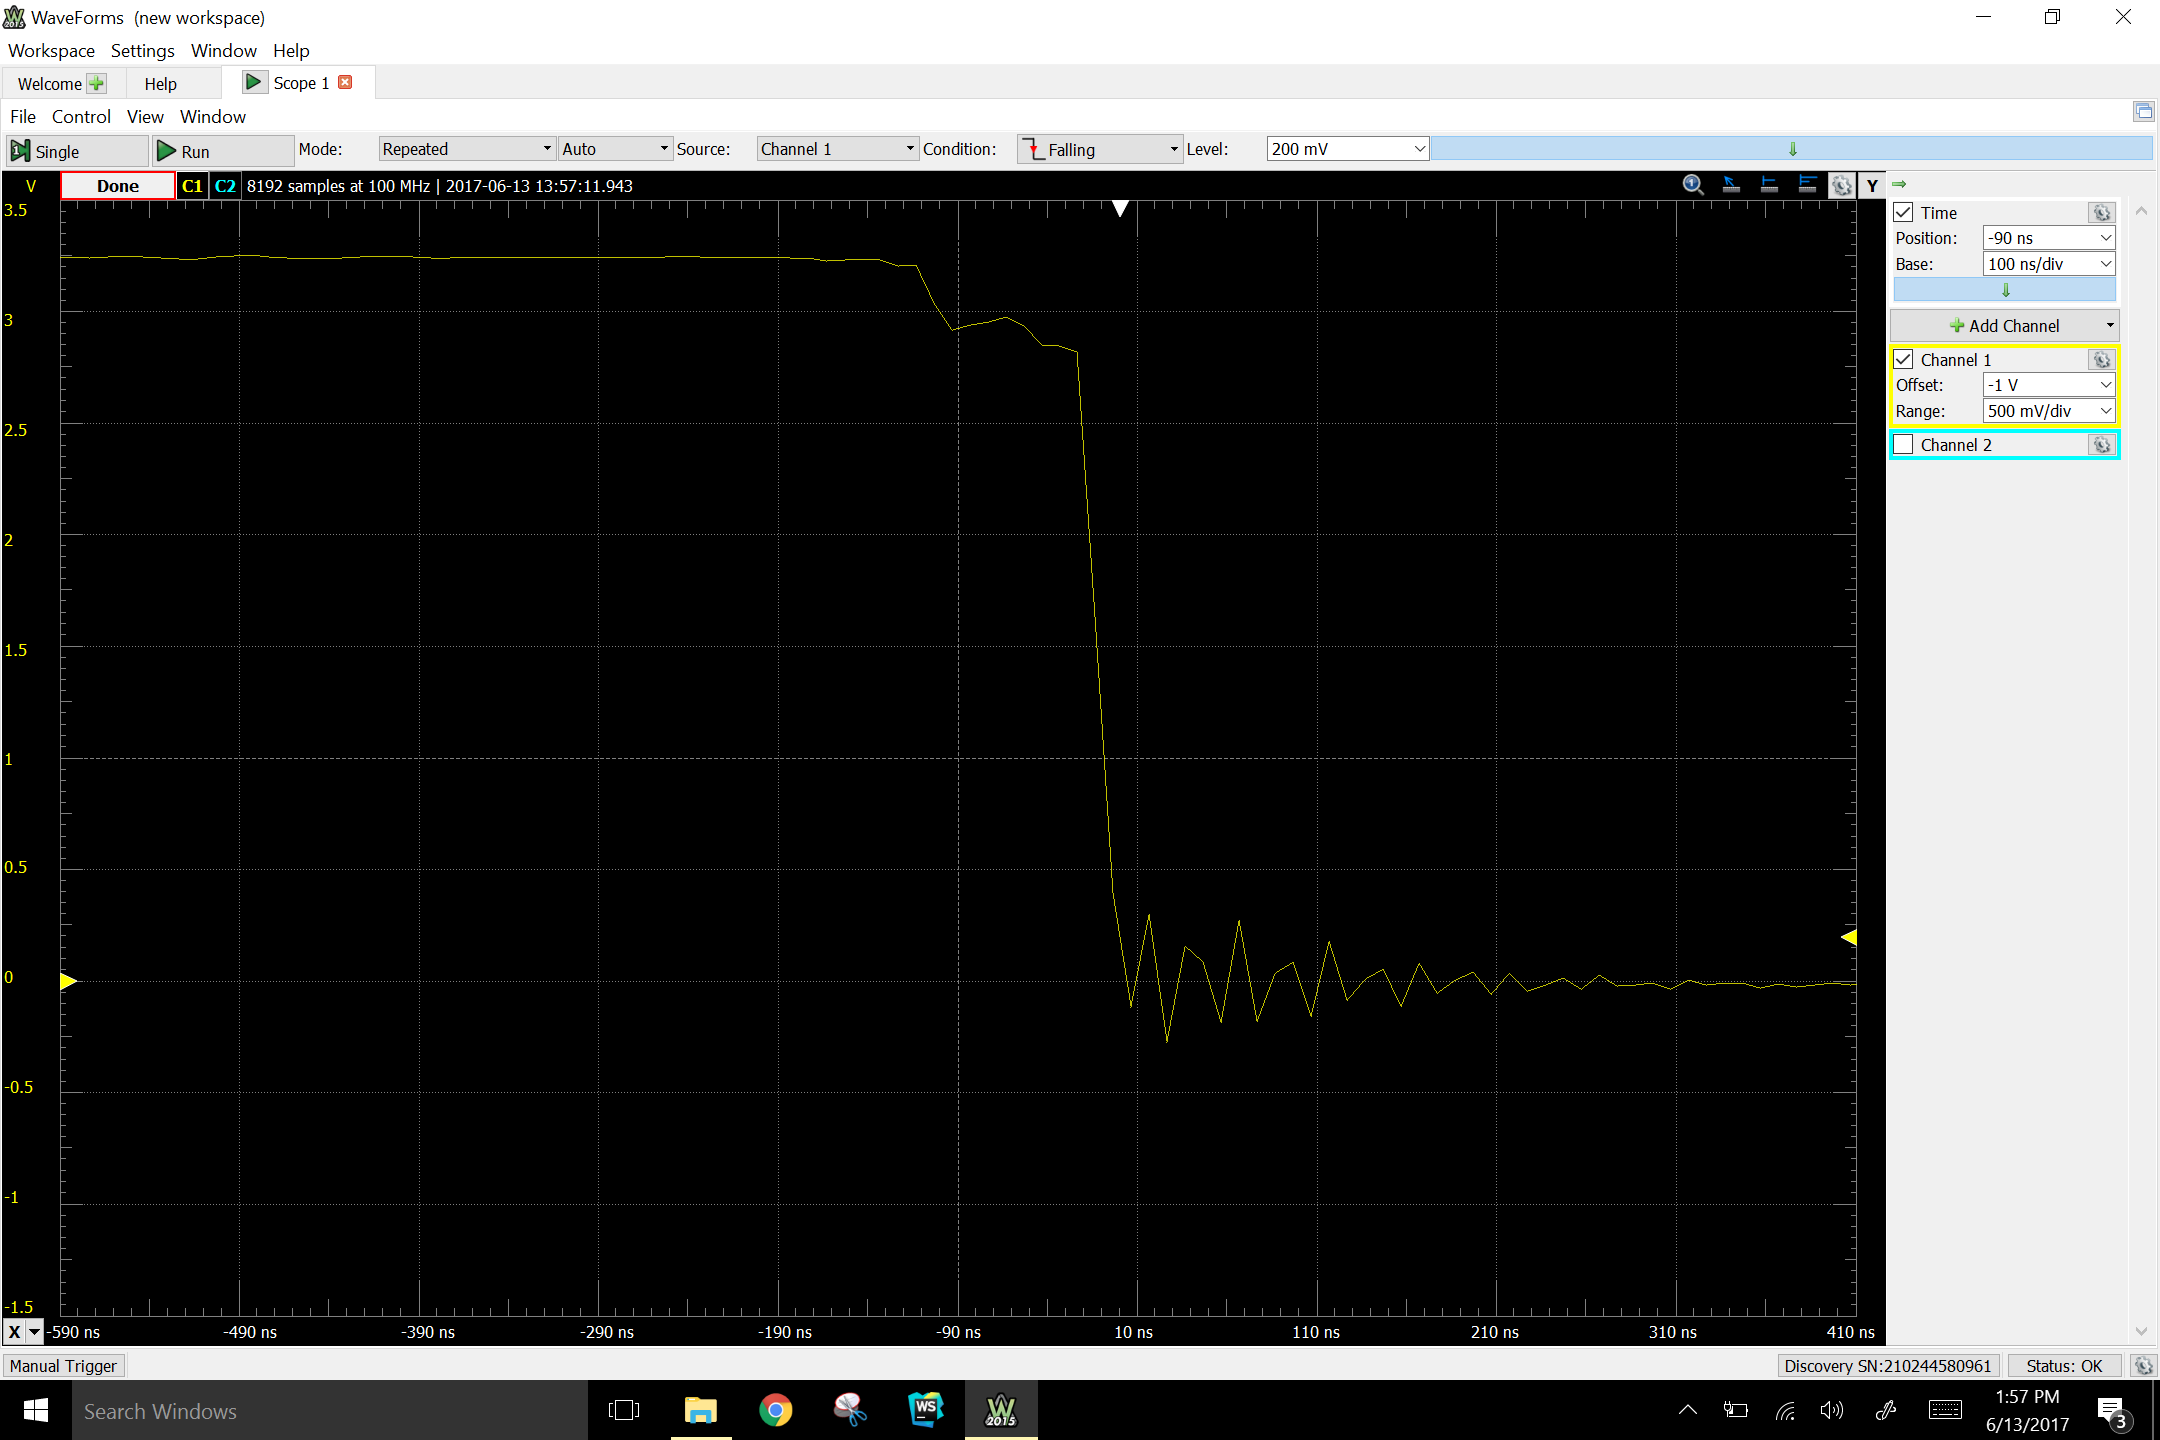
\includegraphics[width=\textwidth]{3b}
	\label{fig:c}
	\caption{DEBOUNCE FALLING EDGE 2}
\end{figure}
\begin{figure}[H]
	\centering
	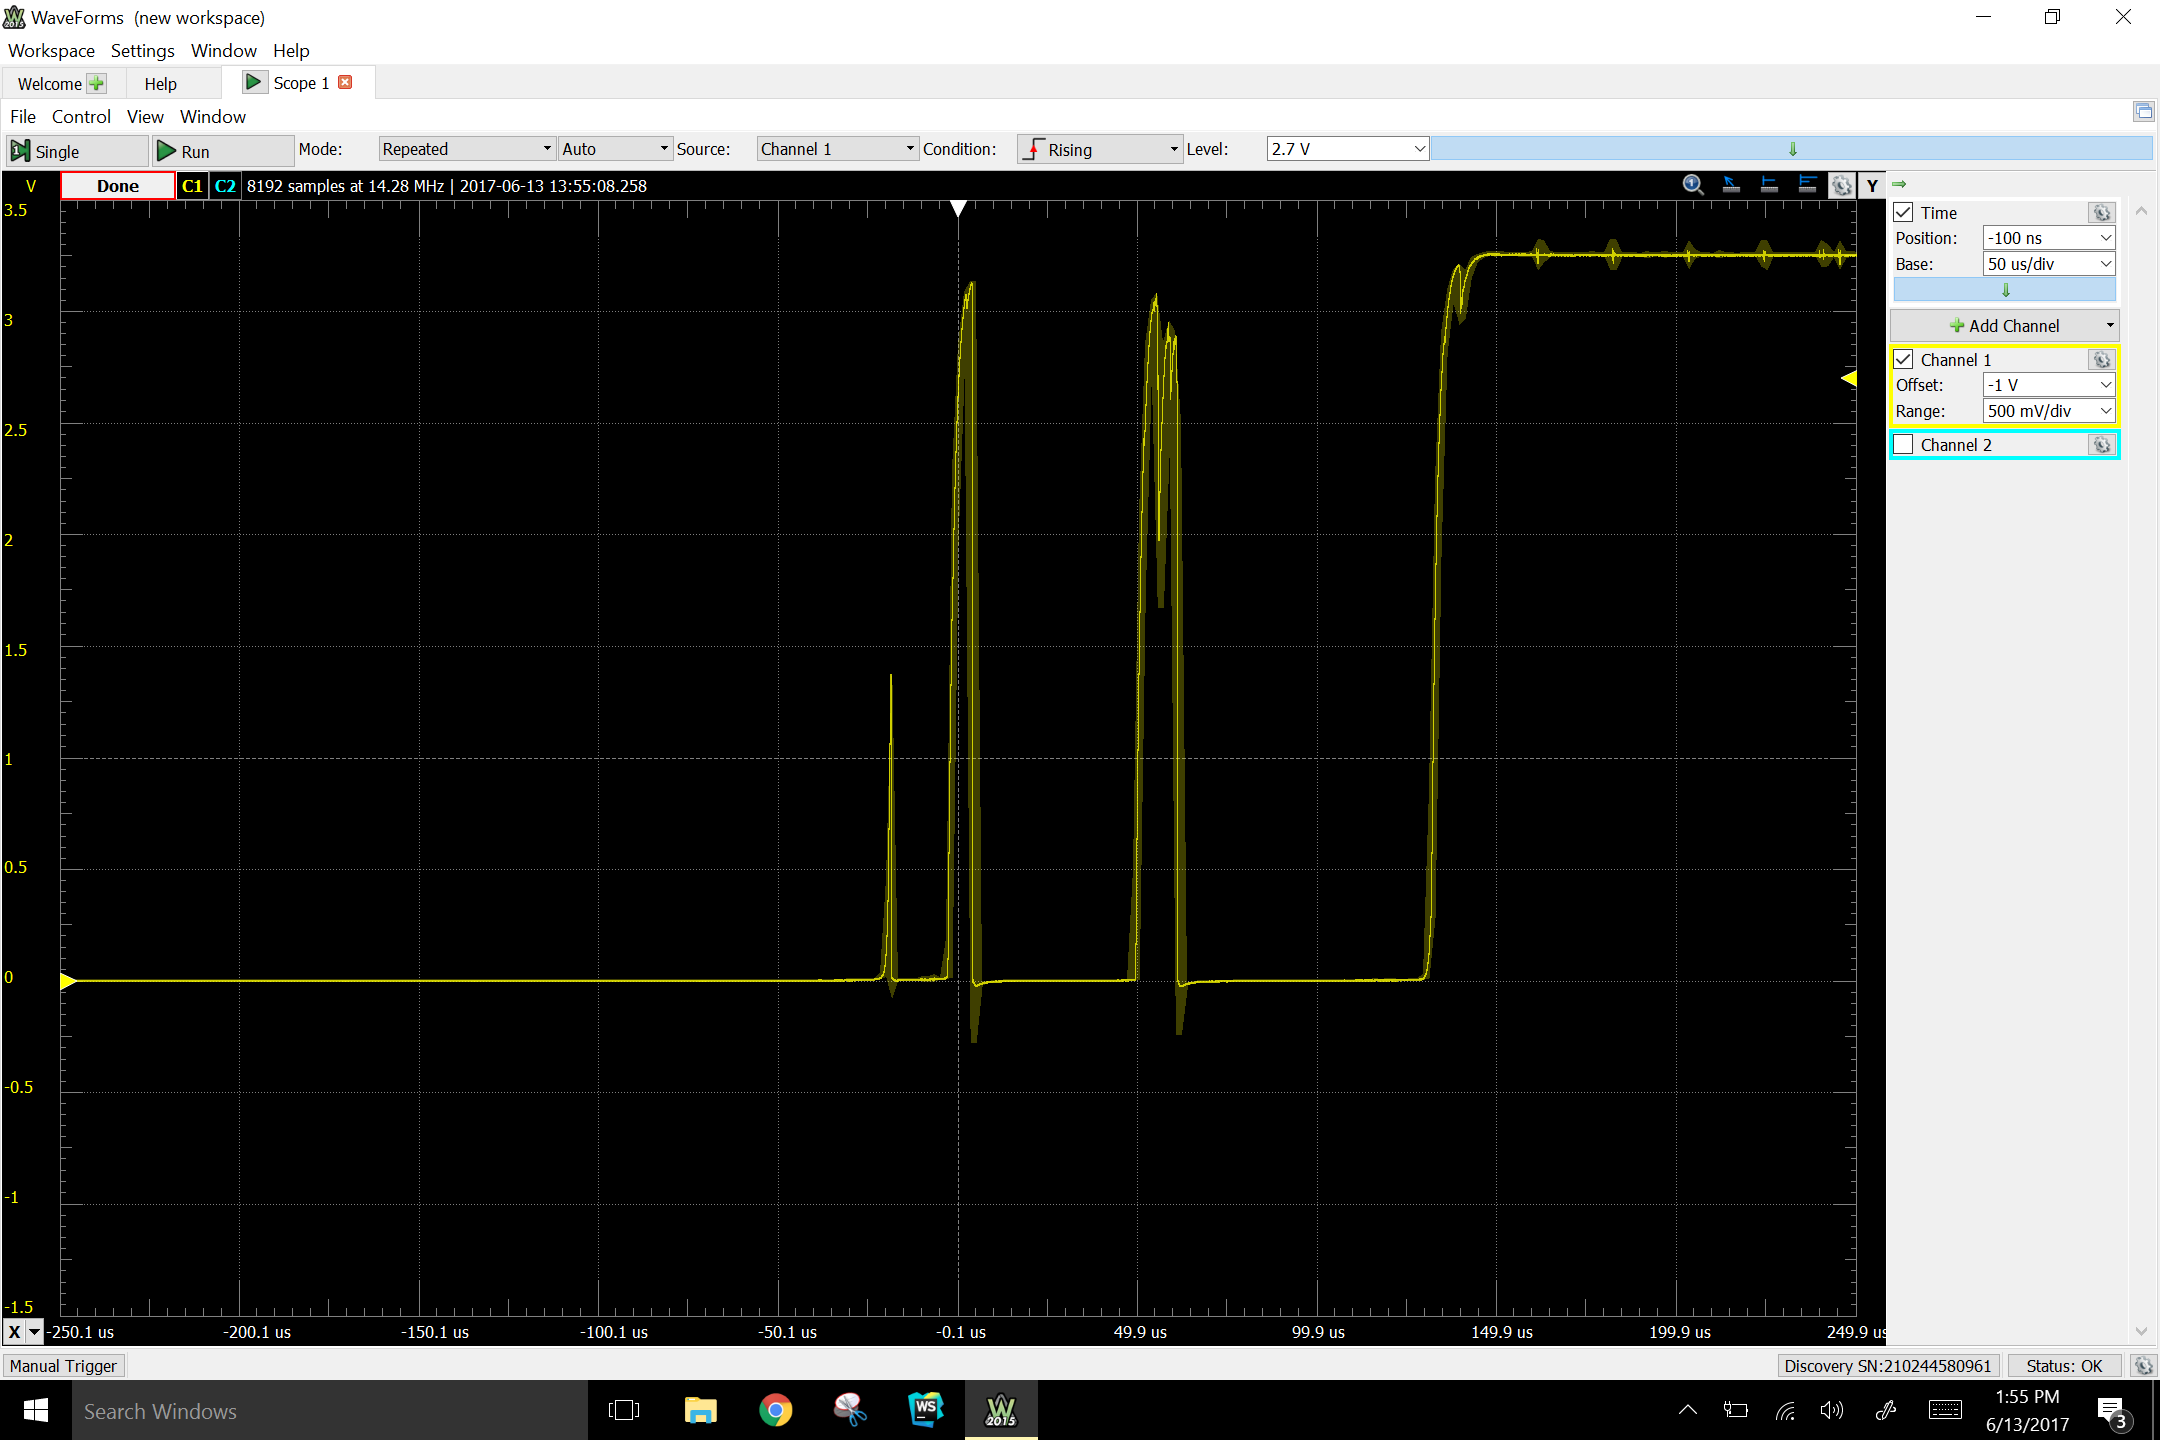
\includegraphics[width=\textwidth]{3c}
	\label{fig:c}
	\caption{DEBOUNCE RISING EDGE 1}
\end{figure}
\begin{figure}[H]
	\centering
	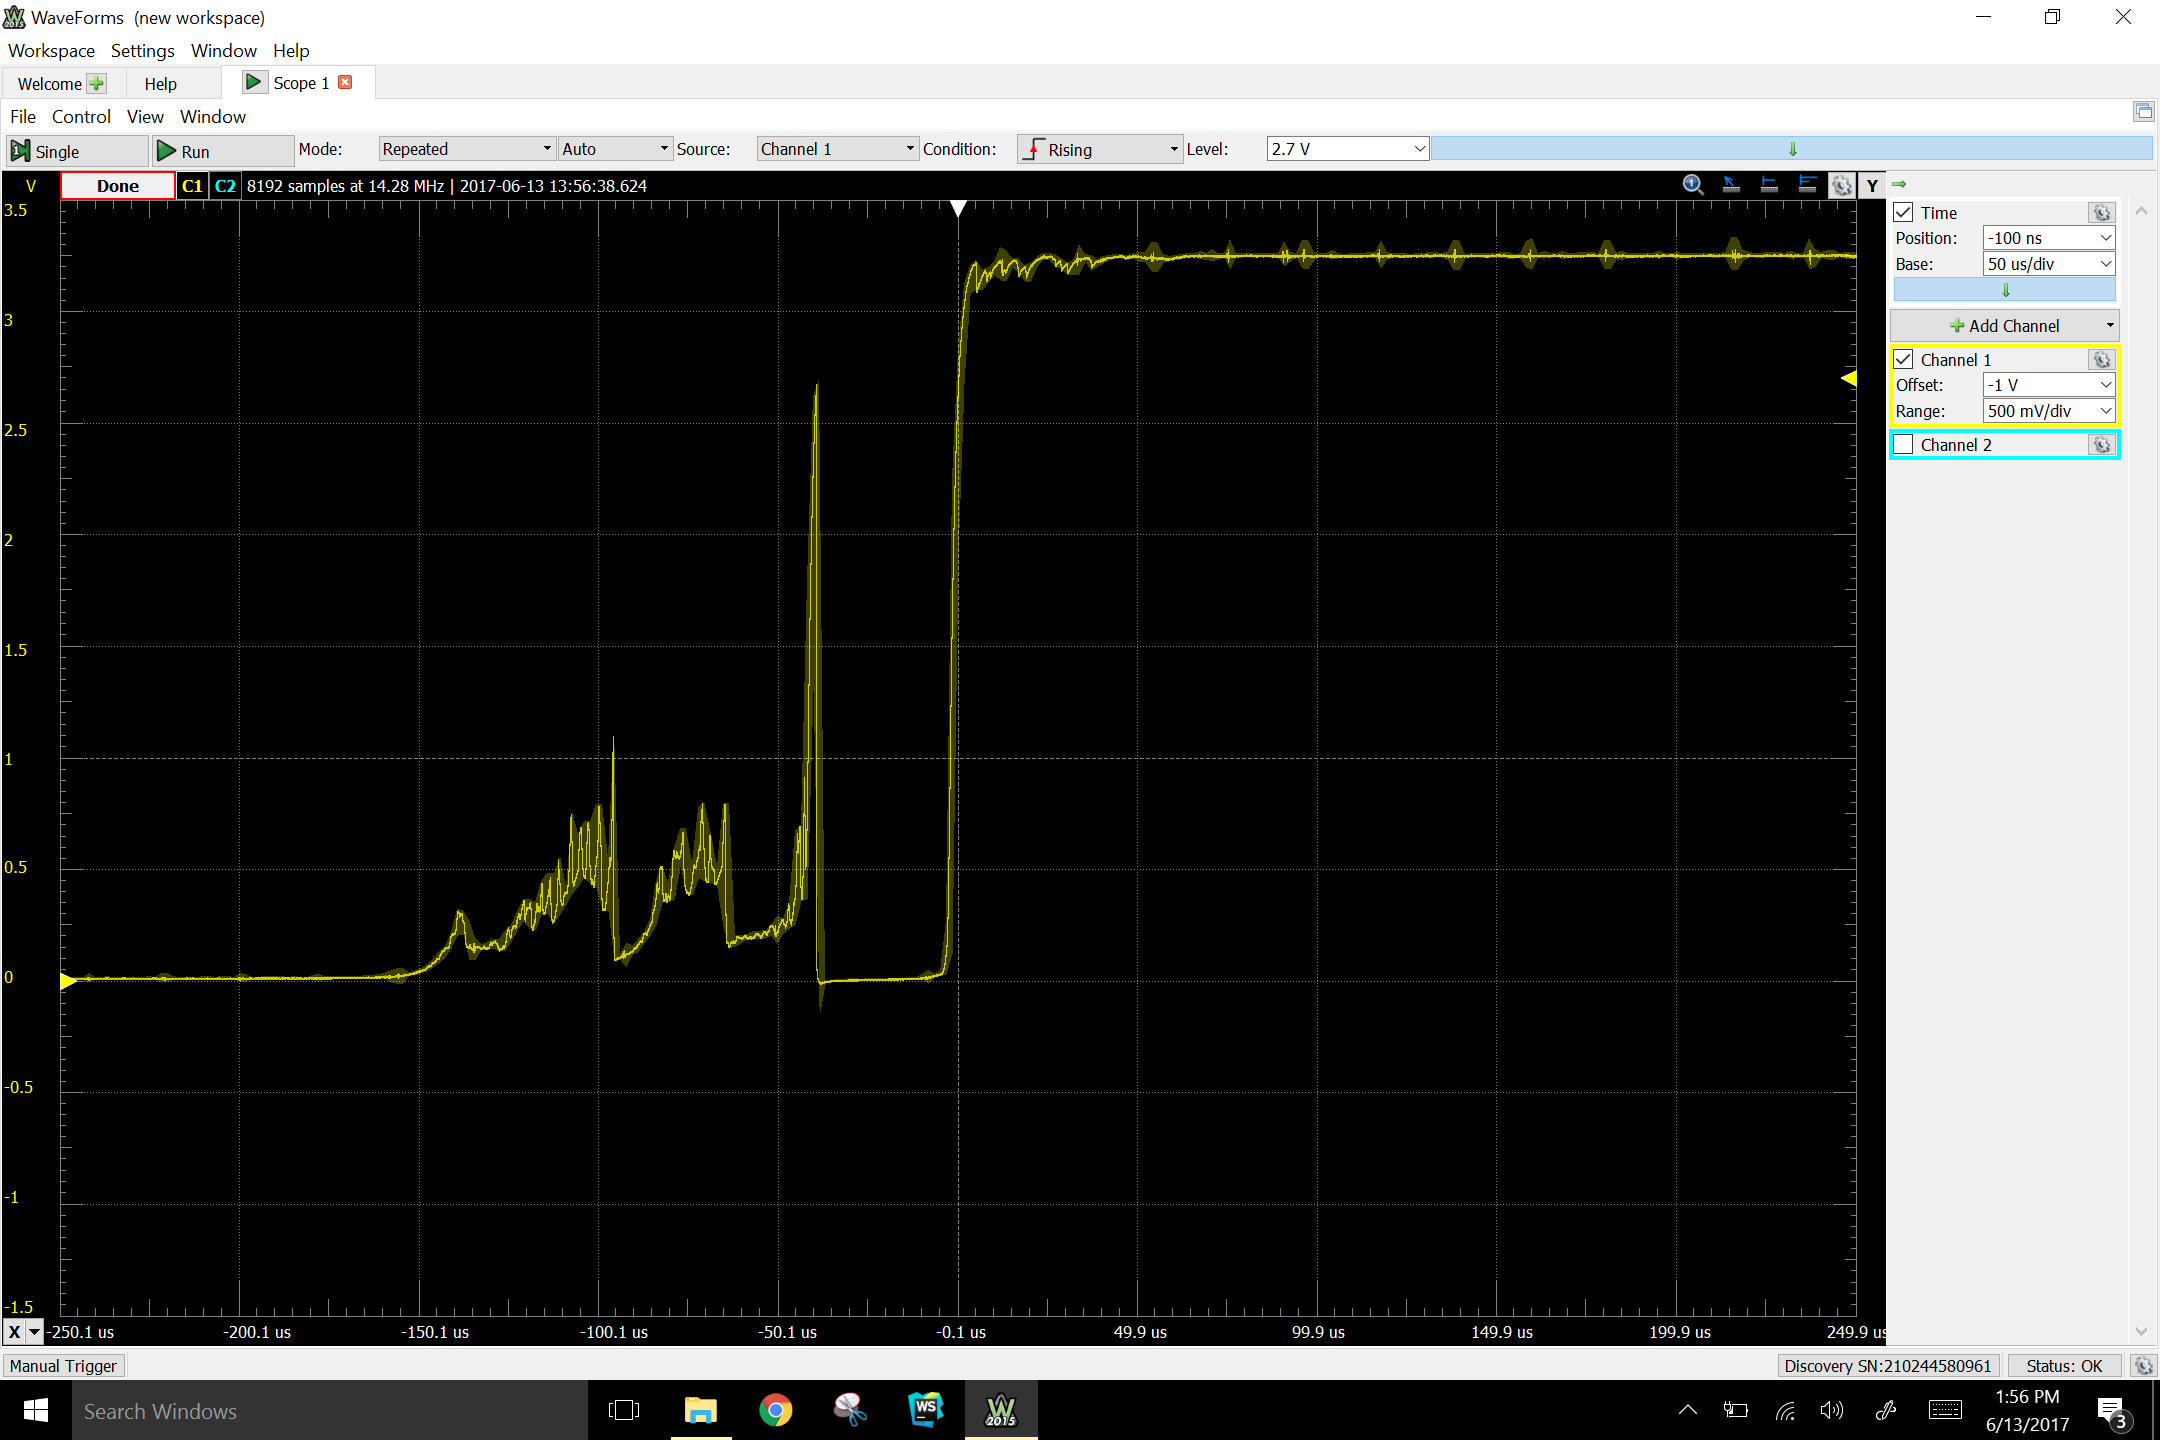
\includegraphics[width=\textwidth]{3d}
	\label{fig:c}
	\caption{DEBOUNCE FALLING EDGE 1}
\end{figure}

THIS WAS ABOUT 100 u seconds. Thus the counter was at least 13
\end{document}